\documentclass{article}
\usepackage[utf8]{inputenc}
\usepackage[autostyle=true]{csquotes}
%\usepackage{hyperref}
\usepackage[hidelinks]{hyperref}
\usepackage[T1]{fontenc}
\usepackage[english]{babel}
\usepackage[utf8]{inputenc}
\usepackage{setspace}
\usepackage{caption}
%\usepackage[margin=1.5cm]{geometry}
\usepackage{geometry}
\geometry{left=15mm,top=20mm, bottom=20mm, right=15mm}
\usepackage{float}
%\usepackage[nottoc,numbib]{tocbibind}
\usepackage{tocloft}
\usepackage{amsmath}
\usepackage{tabu}
\usepackage{float}
\usepackage{wrapfig}
\usepackage{multirow}
\usepackage{gensymb}
\usepackage{graphicx}
\usepackage{rotating}
\usepackage{subcaption}
\usepackage{tasks}
\usepackage{hyperref}
\usepackage{ragged2e}
\usepackage{subcaption}
\usepackage{wrapfig}
\usepackage{xcolor}
\usepackage{chemfig}
\usepackage{mhchem}
\DeclareCaptionType{equ}[][]
\captionsetup[equ]{labelformat=empty} 

\setlength{\parindent}{0cm}
\setcounter{secnumdepth}{5}
\setcounter{tocdepth}{5}
\onehalfspacing
\usepackage{fancyhdr}
\usepackage{etoolbox}
%\usepackage{biblatex}
\usepackage[
    backend=biber, 
    natbib=true,
    style=numeric,
    sorting=none
]{biblatex}
\addbibresource{myReferences.bib}
%\bibliographystyle{unsrt}


\pagestyle{fancy}
\fancyhf{}
\rhead{Mid Term Exercise}
\lhead{ Enrico Turato - Processing and Analysis of Biological Data, BIOS14}
\lfoot{Blossoms Dataset}
\cfoot{\thepage}
\rfoot{2022-DEC-02}

\newcommand{\listequationsname}{List of Equations}
\newlistof{myequations}{equ}{\listequationsname}
\newcommand{\myequations}[1]{%
\addcontentsline{equ}{myequations}{\protect\numberline{\theequation}#1}\par}
\setlength{\cftmyequationsindent}{1.5em}
\setlength{\cftmyequationsnumwidth}{2.3em}
\renewcommand{\cftequtitlefont}{\normalfont\Large\bfseries}

\begin{document}

\begin{wrapfigure}{r}{0.15\textwidth}
    
\includegraphics[width=0.2\textwidth]{LundUniversity_C2line_RGB.png}
\end{wrapfigure}


\iffalse
        \begin{figure}[H]
            \centering
            
\includegraphics[scale=0.3]{LundUniversity_C2line_RGB.png}
        \end{figure}
\fi
        \Large
        \textbf{Blossoms Dataset: UBL and LBL Relation between\\ 9 Populations}
        
        \Large
        Processing and Analysis of Biological Data, BIOS14
        
        \large
        Enrico Turato, Mid Term Exercise\\
        \large
        2022-DEC-02\\ \\
Visit Github to have access to the very poorly organized repository with poor files names containing the code (and in general all the other files related) used for this small analysis exercise: \url{https://github.com/EnricoTurato/Mid_Term_BIOS14.git}.
%\begin{titlepage}
    \begin{center}
        \begin{figure}[H]
            \centering
            
\includegraphics[scale=0.3]{LundUniversity_C2line_RGB.png}
        \end{figure}
        
        \vspace*{1 cm}
        
        \Huge
        \textbf{Blossoms Dataset}
        
        \huge
        \vspace{0.4cm}
        Processing and Analysis of Biological Data\\
        BIOS14
        
        \LARGE
        \vspace{2cm}
        Enrico Turato\\
        
        \LARGE
        \vspace{2cm}
        Mid Term Exercise\\
        
        \Large
        \vspace{3 cm}
        2022-NOV-28
        
        \vspace{1cm}

    \end{center}
\end{titlepage}
%\tableofcontents
%\clearpage
%\listoffigures
%\listoftables
%\listofmyequations
%\clearpage
\section{Introduction}
\subsection{Background and dataset description}
Referring to \cite{paper} and to the lecture notes on the subject, flowers represent an example of integrated phenotypes meaning that usually various parts constituting the flowers will be varying together with each other (covariace different than zero). This is relevant in Biology because these patterns can affect the fit of flowers to their pollinators, among all the other consequences.
\begin{wrapfigure}{r}{0.5\textwidth}
  \begin{center}
    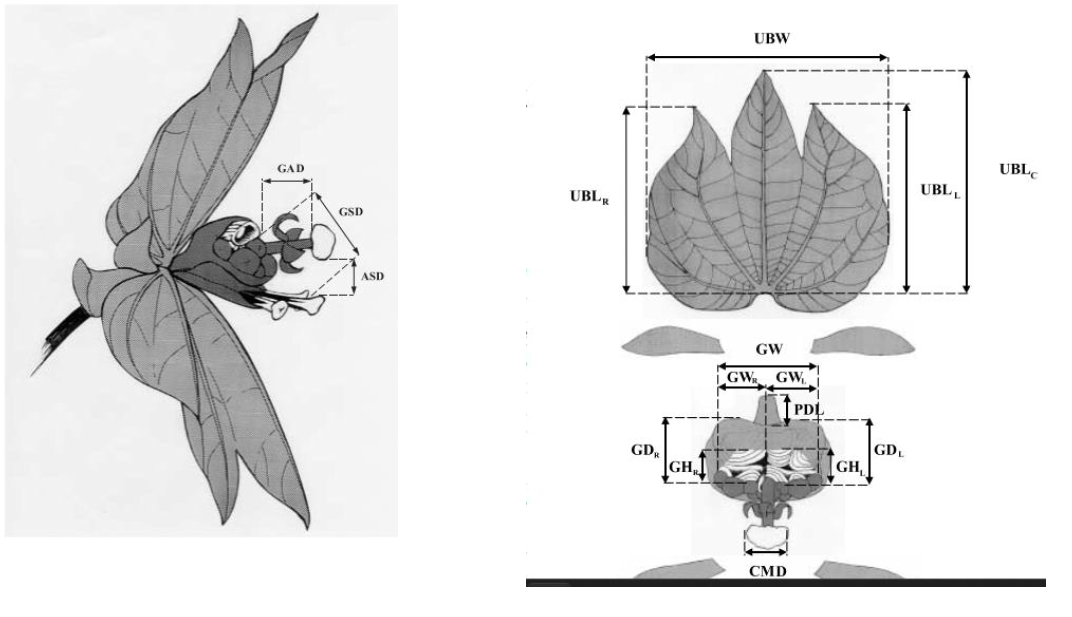
\includegraphics[width=0.48\textwidth]{flower.PNG}
  \end{center}
  \caption{Citing from \cite{paper}, on the left a "side-view of Dalechampia scandens blossom, indicating gland-anther distance (GAD), gland-stigma distance (GSD), and anther-stigma distance (ASD)". On the right, an "exploded view showing remaining floral measurements."}
  \label{fig:flow}
\end{wrapfigure}
More in detail, I will work with a dataset on flower measurements from 9 natural populations in Costa Rica regarding \emph{Dalechampia Blossoms}, \autoref{fig:flow}.
The traits are: ASD: anther-stigma distance (mm); GAD: gland-anther distance (mm); GSD: gland-stigma distance (mm); LBL: lower bract length (mm); LBW: lower bract width (mm); UBL: upper bract length (mm) (The upper and lower
bract lengths are averages of the lengths from the bract base to the tip of the three lobes, \autoref{fig:flow}); UBW: upper bract width (mm); GW: gland width (mm); GA: gland area (mm$^2$).
By referring to the lecture notes: "anther-stigma distance is important for the ability of self-pollination, gland-anther distance and gland-stigmas distance affect the fit of flowers to pollinators, the upper and lower bracts are advertisements (think petals in other flowers), and the gland produces the the reward for pollinators." The chosen traits for this short work are the upper and lower bracts.
\section{Questions and analysis methods}
\paragraph{Hypothesis testing approach:} 
Here I formulate some null hypothesis that I will accept or reject based on the statistical support given by the data by comparing p-values obtained with the chosen alpha = 0.05.
\begin{itemize}
    \item H1: There is no relation between UBL (my chosen response variable) and LBL (my chosen predictor) when considering a randomly chosen population: S1.
    \item H2: The means of observation (UBL) grouped by one factor (populations) are the same.
    \item H3: The means of observation (LBL) grouped by one factor (populations) are the same.
\end{itemize}

\paragraph{Effect sizes approach:}
Estimate the relation between UBL (my chosen response variable) and LBL (my chosen predictor) (if any) for all populations. Give also information on the variances explained by and within populations.


\subsection{Chosen methods per approach}
\begin{enumerate}
    \item[2.0.0.1] I will perform a linear regression on S1 (reg = lm(UBL $\sim$ LBL)), check residuals and summary table and then a one-way ANOVA analysis (aov(UBL $\sim$ populations, data = dat) and aov(LBL $\sim$ populations, data = dat)) (even though with a categorical variable, populations) and check the summary table. I will compare p-values with 0.05.
    \item[2.0.0.2] I will use an ANCOVA analysis (ancv = lm(UBL $\sim$ -1 + populations + LBL:populations, data = dat) to obtain the slopes for UBL vs LBL (coef(ancv)) for all the populations and the variances among and within populations by using a linear mixed model (m = glmmTMB(UBL $\sim$ LBL + (1|populations), data=dat)) with random effect the populations.
\end{enumerate}
\section{Results and Conclusions}
\begin{figure}[H]
\centering
  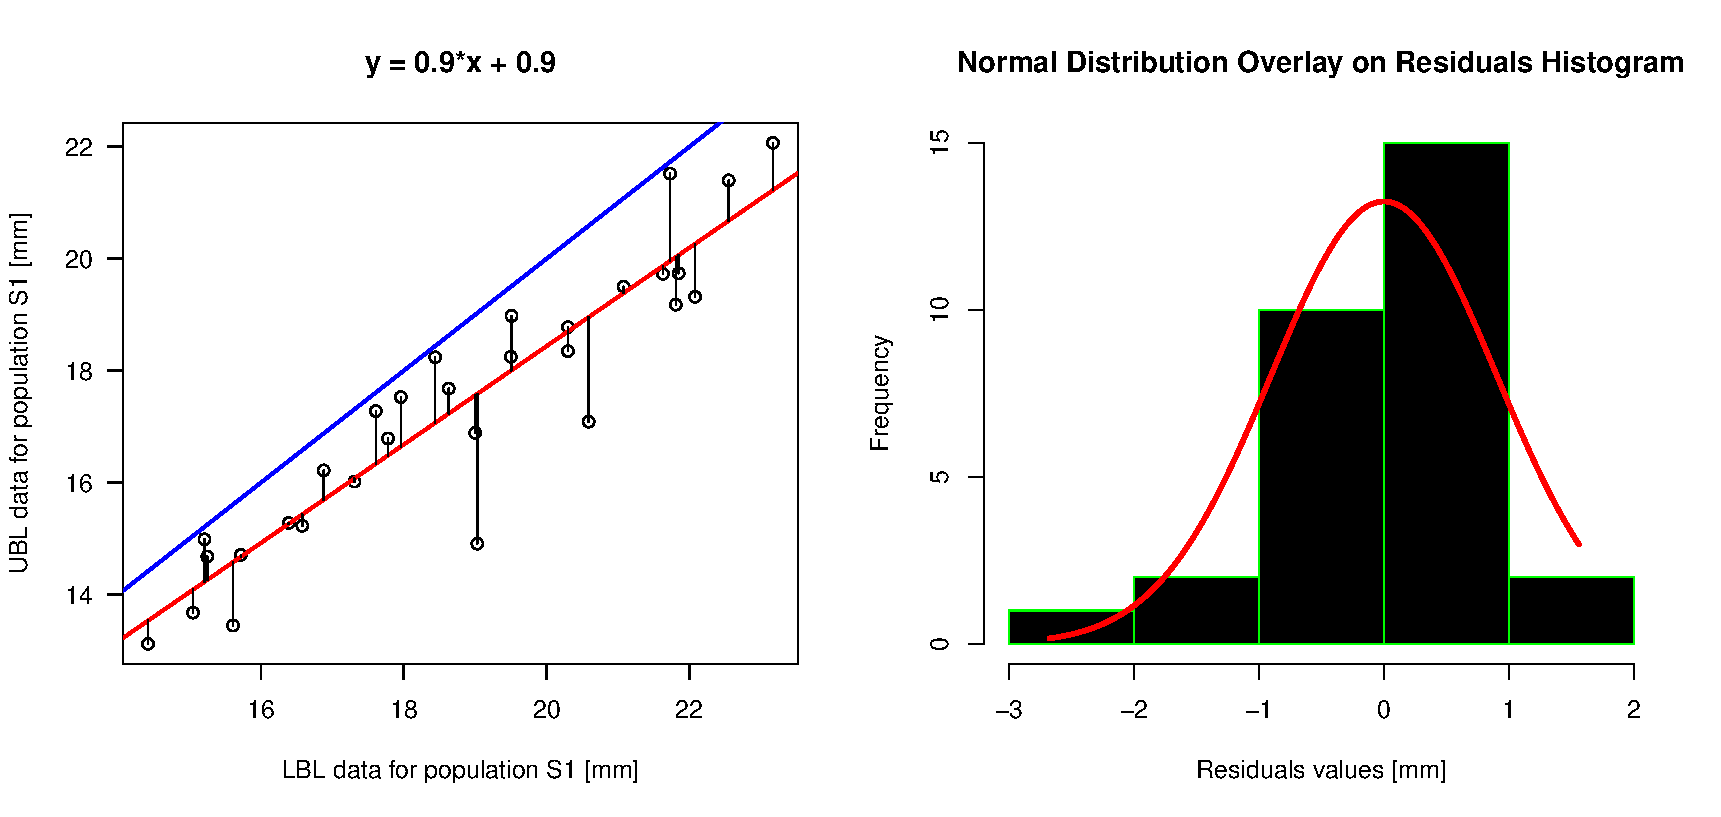
\includegraphics[scale=0.4]{reg_S1.pdf}
\caption{On the left, the linear regression graphical results on S1 (red line, the lower) with a 1:1 blue line showing y = x + 1. On the right the values of the residuals on the x-axis [mm] vs their frequency and a normal distribution overlay.}
  \label{fig:regS1}
\end{figure}
Considering the population S1, \autoref{fig:regS1}: the residuals obtained after performing a linear regression are normally distributed as wanted. For +1 mm change in LBL, the UBL will change by +0.9 mm (rounded) (slope: 0.88 mm/mm $\pm$0.07 mm/mm). The null hypothesis H1 can be rejected, F-statistic$_{1, 28}$ = 174.6 and  P < 0.0001 : there is enough statistical support to believe in the existence of a linear relation between the response variable, UBL, and the predictor, LBL. R-squared = 0.8618 meaning $\approx$ 86\% of the variance in y is explained by x.
Now taking a look at all the populations, let's first inspect how the values for UBL and LBL are distributed when putting together all the data, \autoref{fig:distribu}.
\begin{figure}[H]
\centering
  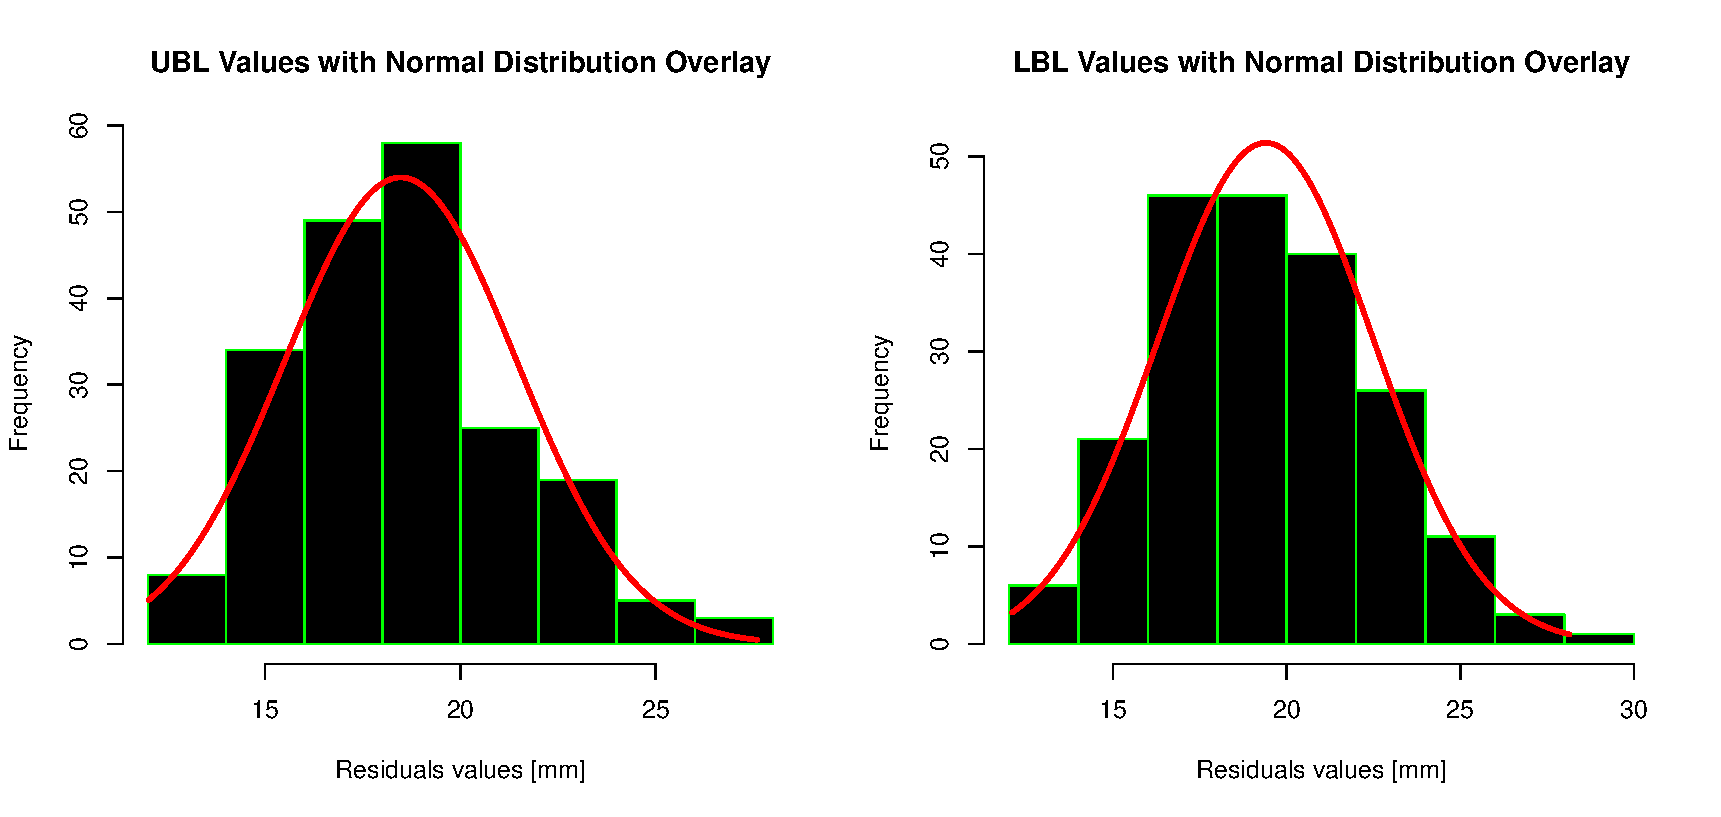
\includegraphics[scale=0.45]{ubl_lbl-distr.pdf}
\caption{Graphical representation of normally distributed values across the populations for UBL ad LBL.}
  \label{fig:distribu}
\end{figure}
By looking now, instead, at the populations individually but on the same plots with boxplots, I have the following \autoref{fig:boxplots}.
\begin{figure}[H]
     \centering
  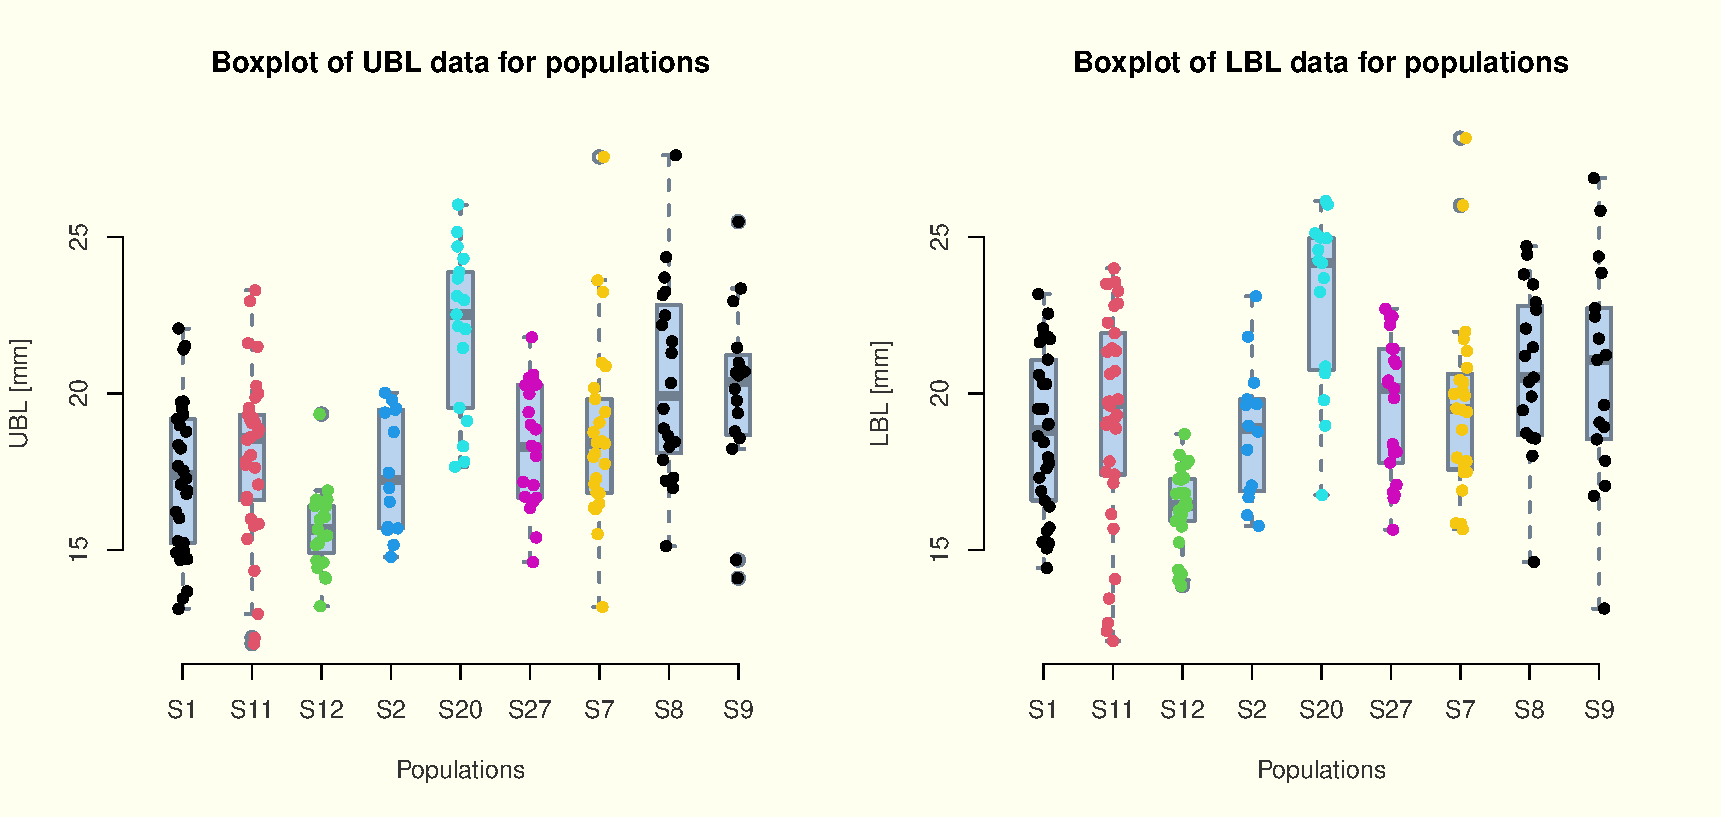
\includegraphics[scale=0.65]{ubl_lbl-popu.pdf}
     \caption{Variations of UBL (left) and LBL (right) grouped by populations.}
     \label{fig:boxplots}
\end{figure}

The values for the mean, standard deviation and standard error for each population, both for UBL and LBL are summarized in the following \autoref{tab:values}.

\begin{table}[H]
\centering
\caption{Relevant values for the populations.}
\begin{tabular}{c c c c c c c } 
 \hline
Population & UBL Mean [mm] & UBL SD [mm] & UBL SE [mm] & LBL Mean [mm] & LBL SD [mm] & LBL SE [mm]    \\  
 \hline
 S1 &17.35&2.43&0.44&18.77&2.57&0.47 \\
 S11 &18.03&2.68&0.46&19.23&3.44&0.59 \\
 S12 &15.68&1.26&0.26&16.37&1.28&0.26 \\
 S2 &17.50&1.93&0.52&18.77&2.15&0.58 \\
 S20 &22.02&2.65&0.64&22.94&2.84&0.73 \\
 S27 &18.30&1.94&0.41&19.59&2.19&0.47 \\
 S7 &18.74&2.94&0.59&19.61&2.95&0.60 \\
 S8 &20.41&3.11&0.70&20.74&2.61&0.60 \\
 S9 &19.99&2.88&0.72&20.65&3.56&0.86 \\
 \hline
\end{tabular}
\label{tab:values}
\end{table}

I will now briefly cover the results of one-way ANOVA analysis of UBL and LBL vs populations.
Both the null hypothesis H2 and H3 can be rejected: F-value$_{8, 192}^{UBL}$ = 11.345 and F-value$_{8, 191}^{LBL}$ = 8.370 with both P < 0.0001. There is enough statistical support to believe that both means of observation, UBL and LBL, when grouped by populations, show some differences. To better quantify, instead, the variance explained by the populations and the variance within populations I now perform the above-mentioned linear mixed model with the populations as random effect, \autoref{tab:values2}.

\begin{table}[H]
\centering
\caption{Relevant values for the populations.}
\begin{tabular}{c c c c c c c } 
 \hline
 Mean LBL [mm]& LBL SD [mm]&Var. among Pop. [\%]&Var. within Pop. [\%]&CV among& CV within& Tot CV  \\  
 \hline
 19.400&3.106&16.235&83.765&0.001&0.003&0.004 \\
 \hline
\end{tabular}
\label{tab:values2}
\end{table}
As wanted, the variance explained by the model among populations, 16.2\% is lower than the "mean" variance explained by the model within populations, 83.8\%.

I can now perform also an ANCOVA analysis to obtain all the slopes and intercepts of linear regressions between UBL and LBL for each population, \autoref{tab:values3}.
\begin{table}[H]
\centering
\caption{Obtained (rounded) intercepts and slopes values for the populations.}
\begin{tabular}{c c c} 
 \hline
Population & Intercepts [mm] & Slopes [mm/mm] \\  
 \hline
 S1 &0.86&0.88 \\
 S11 &4.7&0.69 \\
 S12 &2.5&0.80 \\
 S2 &3.0&0.77 \\
 S20 &4.0&0.80 \\
 S27 &3.5&0.75\\
 S7 &4.6&0.70 \\
 S8 &-0.07&0.97 \\
 S9 &4.3&0.75\\
 \hline
\end{tabular}
\label{tab:values3}
\end{table}
Both the interactions and the main effect are statistically supported (P < 0.0001) meaning that both the slopes and intercepts differ between populations when considering the linear relation between the response variable, UBL, and the predictor, LBL .

\iffalse
> #######################################################################
> # getting slopes from mixed models approach
> #######################################################################
different compared to before because:
In statistics, best linear unbiased prediction (BLUP) is used in linear mixed models for the estimation of random effects.


mmmm = glmmTMB(y ~ x +(x|populations), data=dat)
> 
> coef(mmmm)

    (Intercept)         x
S1     2.392067 0.8061888
S11    3.793606 0.7390777
S12    2.600621 0.8021841
S2     2.962262 0.7817197
S20    1.547531 0.8943891
S27    3.018563 0.7821726
S7     3.418051 0.7615902
S8     1.458555 0.8908987
S9     2.646788 0.8209915
\fi
Given what I observed, now I can also do a linear regression by putting all populations together:

\begin{figure}[H]
\centering
  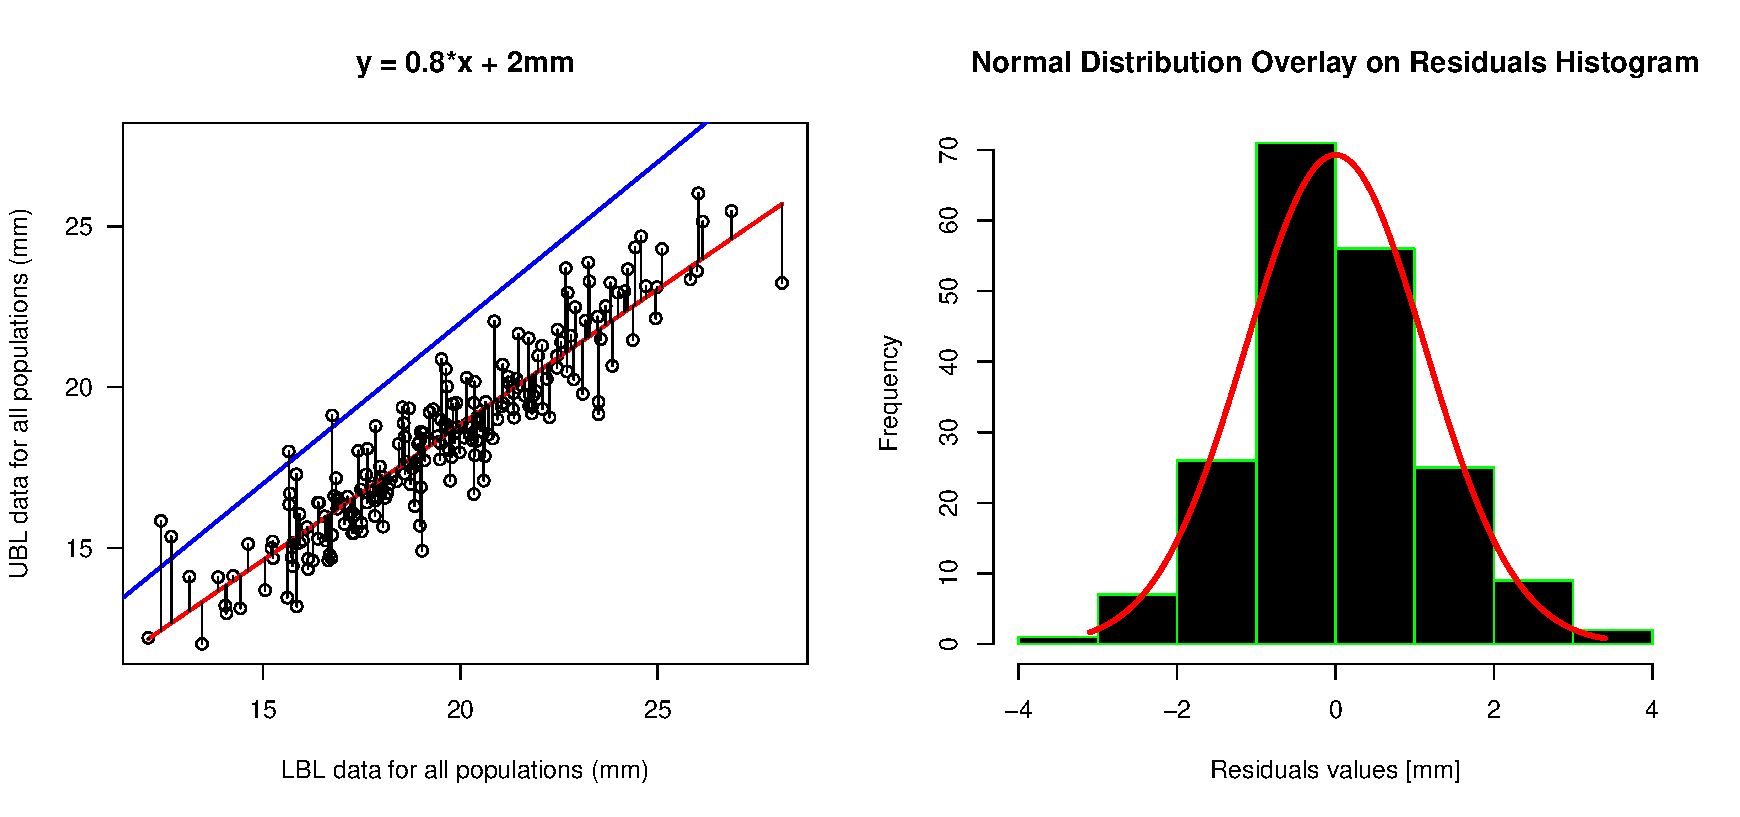
\includegraphics[scale=0.6]{full_reg.pdf}
\caption{Linear regression graphical results on all the populations.}
  \label{fig:fullregS1}
\end{figure}

Considering all the populations: the residuals obtained after performing a linear regression are normally distributed. For +1 mm change in LBL, the UBL will change by +0.8 mm (rounded) (slope: 0.84 mm/mm $\pm$ 0.03 mm/mm). A similar null hypothesis to H1 (applied this time to all the populations mixed) can be rejected, F-statistic$_{1, 195}$ = 1033 and  P < 0.0001 : there is enough statistical support to believe in the existence of a linear relation between the response variable, UBL, and the predictor, LBL, when considering all the populations together. R-squared = 0.8412 meaning $\approx$ 84\% of the variance in y is explained by x.\\ 
\AtNextBibliography{\footnotesize}
\printbibliography

\end{document}
